% book example for classicthesis.sty
\documentclass[
  % Replace twoside with oneside if you are printing your thesis on a single side
  % of the paper, or for viewing on screen.
  %oneside,
  oneside,
  11pt, a4paper,
  footinclude=true,
  headinclude=true,
  cleardoublepage=empty
]{scrbook}
%\usepackage{array}
%\usepackage{lipsum}
\usepackage[linedheaders,parts,pdfspacing]{classicthesis}
\usepackage{amsmath}
\usepackage{amsthm}
\usepackage{hyperref}
\usepackage{graphicx}
\usepackage{listings}

\usepackage{array}

\usepackage[utf8]{inputenc}
\usepackage[T1]{fontenc}
\usepackage{eurosym}
\newcommand{\intervalle}[4]{\mathopen{#1}#2
 \mathclose{}\mathpunct{};#3
 \mathclose{#4}}
\newcommand{\intervalleff}[2]{\intervalle{[}{#1}{#2}{]}}
\newcommand{\intervalleof}[2]{\intervalle{]}{#1}{#2}{]}}
\newcommand{\intervallefo}[2]{\intervalle{[}{#1}{#2}{[}}
\newcommand{\intervalleoo}[2]{\intervalle{]}{#1}{#2}{[}}

\title{Simulation d’une équipe de robots pompiers - TP en temps Libre}
\author{Salah-Eddine Bariol Alaoui\\Majd Fariat\\Dimitri Pierucci}

\begin{document}

\maketitle

%\include{FrontBackMatter/abstract}
%\include{FrontBackMatter/dedication}
%\include{FrontBackMatter/acknowledgements}
%\include{FrontBackMatter/declaration}
%\include{FrontBackMatter/contents}

%\part{Introduction}

\chapter{Première partie : les données du problème}

La première partie du TP, correspond en la réalisation des classes Java représentant le problème et du simulateur. \\

Nous avons séparé les entités en quatre packages. \\

\begin{tabular}{|c|c|}
	\hline Package & Robot \\
	\hline \hline 
	classes & Drone \\
			& Robot \\
			& RobotAChenilles \\
			& RobotAPattes \\
			& RobotAroues \\
			& RobotReservoir \\
			& RobotTerrestre \\
	\hline \hline
	Package & Géographie \\
	\hline \hline
	classes & Carte \\
			& Case \\
			& EnumDirection \\
			& EnumNatureTerrain \\
			& Incendie \\
	\hline \hline
	Package & Simulation \\
	\hline \hline
	classes & DonneesSimulation \\
			& Simulateur \\
	\hline \hline
	Package & io \\
	\hline \hline
	classes & LecteurDonnees \\
	\hline
\end{tabular} \\

\section{Package Robot}
Le package Robot contient la classe abstraite Robot ainsi que toutes les classes l'implémentant. \\ 

Nous avons cherché à optimiser l'implémentation des sous-classes de Robot en factorisant le plus possible. \\ 

%Les classes Drone, RobotAChenilles et RobotAroues ont la particularité d'avoir un réservoir contrairement à RobotAPattes. Nous les avons donc leurs points communs dans une classe abstraire RobotReservoir fille de Robot. \\

%RobotAChenilles et RobotAroues sont différend de Drone, Ils ont une diminution de la vitesse en rapport à la Case où ils se situent et ne vident pas leur réservoir de la même façon de Drone. Nous avons regroupé leurs points communs dans une sous-classe abstraire RobotTerrestre fille de RobotReservoir. \\

Le diagramme UML correspondant du package Robot est le suivant \\

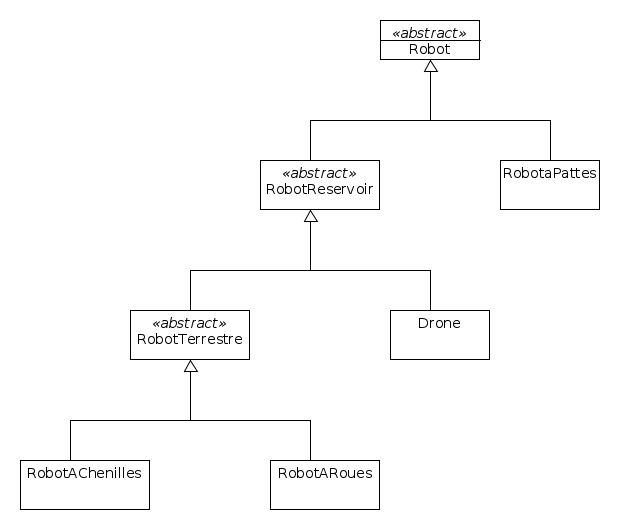
\includegraphics[scale=0.5]{./UML-Robot.jpg}


\section{Autres Packages}
Il n'y a pas vraiment de choix de conception à faire pour les autres packages, la partie 1 est très guidée. 


\chapter{Troisième partie : le plus court chemin}
Pour trouver le plus court chemin, notre algorithme commence par initialiser la distance entre le robot et l'incendie par une valeur maximale. \\

Ensuite, il teste dans une boucle sur les cases accessibles laquelle est la plus proche. Si elle permet de diminuer la distance entre le robot et la destination alors on met la nouvelle distance dans la variable dist et on continue. \\

Dans le cas où la variable 'dist' n'a pas changer de valeur, celà indique que le robot ne trouve jamais une case où il peut se déplacer. On affiche alors le message indiquant que le robot est bloqué.



\chapter{Quatrième partie : Stratégie d'intervention}
On a opté pour la stratégie élémentaire. Il s'agit de parcourir dans 2 boucles imbriqués les incendies qui sont sur la carte, et de parcourir pour chaque incendie la liste des robots pour voir lequel est disponible
\end{document}



























